\documentclass{ledger}

\usepackage{hyperref}
\usepackage{booktabs}
\usepackage{array}
\usepackage{geometry}
\usepackage{longtable}
\geometry{a4paper, margin=1in}
\usepackage{tabularx}

%AUTHOR: This is a bare-bones template into which you may put your paper to aid in formatting your submission to Ledger. Note that to work properly, you must have the files "ledger.cls", "ledgerbib.bst", and the folder "images" on hand. 

%AUTHOR: the preferred method to generate PDF output is to use 'pdflatex'
%To clean up after a successful build, try: 'latexmk -c main.tex'

%EDITOR: in ledger.cls replace logoNewUC.png with logoNew.png prior to publication 


%EDITOR: replace X's to set the data for the header and footer
\newcommand{\thefirstpagenum}[0]{X}
\newcommand{\thelastpagenum}[0]{X}
\newcommand{\theyear}[0]{20XX}
\newcommand{\thevol}[0]{X}
\newcommand{\thedoi}[0]{DOI 10.5195/LEDGER.\theyear.XXX}
\newcommand{\ledgerpages}[0]{\thefirstpagenum-\thelastpagenum}


%AUTHOR: please set these to generate correct PDF metadata
\hypersetup{pdfauthor={Sun, Ephraim T.; 
Gijsbertsen, Laurens C.}, pdftitle={A Study on State-of-the-Art Alternative Asset Models and Their Application to Digital Assets}}

%EDITOR: set the correct pageination during layout
%\setcounter{page}{\thefirstpagenum}


%AUTHOR: this can be used to highlight changed text, surround with \edit{} and
%uncomment either to determine color
%\newcommand{\edit}[1]{{\color{red} #1}}
\newcommand{\edit}[1]{#1}
	
\overfullrule=10pt

\title{A Study on State-of-the-Art Alternative Asset Models and Their Application to Digital Assets
}
\author{Dr. Simon Mak\thanks{S. Mak (smak@smu.edu) - Faculty Advisor, Director of the Caruth Institute for Entrepreneurship}, Ephraim T. Sun\thanks{E. Sun (ephraims@smu.edu)} , Laurens C. Gijsbertsen,\thanks{L. Gijsbertsen (lgijsbertsen@smu.edu)}}

\pagestyle{pagemain}


%The Author should select the appropriate pretitle below:
\pretitle{
  \centering \selectfont LEDGER \LaTeX \ TEMPLATE \par
  %\centering \selectfont REVIEW ARTICLE \par
  %\centering \selectfont RESEARCH ARTICLE \par 
  %The Author should not remove the following text:
  Submission Under Consideration at Ledger \par 
  \fontsize{24pt}{28pt}\selectfont} % Title is centered and at 24pt


\begin{document}

\maketitle

\thispagestyle{pagefirst}

\begin{abstract}
This research project aims to conduct a comprehensive study on state-of-the-art alternative asset models and their application to digital assets. As the financial landscape continues to evolve, alternative assets, specifically digital assets, are gaining significant attention, and becoming increasingly relevant for investors. However, there is a lack of rigorous research and understanding of the various alternative asset investment models and their implications for digital assets. The primary research question driving this study is: "\textit{To what extent can existing alternative asset investing models be applied to digital assets?}" By examining and analyzing various alternative asset models, this research project seeks to assess the feasibility and effectiveness of applying these models to digital assets.

%AUTHOR: keywords are OK to show for Review article, will be hidden and added to metadata for publication
\begin{keywords}
\item State-of-the-art.
\item Alternative asset models.
\item Digital assets.
\item Cryptocurrency.
\item Application.
\item Feasibility.
\item Effectiveness.
\item Portfolio theory.
\item Factor-based models.
\item Risk management.
\end{keywords}
\end{abstract}

\section{Introduction}
\subsection{Background}
Digital assets have grown rapidly in recent years, with the total market cap of cryptocurrencies surpassing \$2 trillion in 2021. While digital assets hold promising investment opportunities, the volatile and decentralized nature of this new asset class presents unique investment challenges compared to traditional assets. As investor interest in digital assets continues to grow, there is a need to explore best practices for evaluating and managing risks associated with digital asset investments.

Alternative asset investing offers strategies that may help address some of the challenges with digital assets. However, applying traditional alternative asset models directly to digital assets is not straightforward given key differences in their characteristics. It is therefore important to examine existing models and understand how they may need to be adapted for the digital asset landscape.

\subsubsection{Alternative Asset Models}
A wide range of alternative asset investing models have been developed and applied across various private market asset classes such as private equity, private credit, real assets and hedge funds. Common models used include portfolio theory, factor models, mean-variance optimization, and risk parity frameworks.

While these models have proven valuable in traditional alternative investments, it remains unclear whether and how they can be applied to digital assets. Digital assets such as cryptocurrencies differ significantly from traditional assets in factors like volatility, liquidity profile and regulatory oversight (FINRA.org).

\subsection {Digital Assets}
Cryptocurrencies were the first widely adopted digital assets, with Bitcoin being the largest. Since then, new digital asset classes have emerged including security tokens representing asset ownership, and utility tokens providing access to a network or platform.

Digital assets present both opportunities and challenges from an investment perspective. While some studies show they can provide portfolio diversification benefits, their short history makes volatility and risk difficult to assess over long periods (FINRA.org). Regulatory ambiguity also introduces legal and compliance complexities for investors (CRS Reports, 2023).

Connecting these concepts, there is a need for research exploring whether and how existing alternative asset investing approaches could benefit the growth of a regulated digital asset investment industry. This paper aims to address this gap by systematically analyzing various models and evaluating their applicability to different digital asset classes.

\section{Overview of Existing Alternative Asset Models and Their Key Principles}

% \begin{itemize}
%        \item[1] Risk and Return Analysis
%             \begin{itemize}
%             \item[1.1] Capital Asset Pricing Model (CAPM)
%             \end{itemize}
%        \item[2] Volatility Analysis
%             \begin{itemize}
%             \item[2.1] Generalized AutoRegressive Conditional Heteroskedasticity (GARCH)
%             \item[2.2] Stochastic Model - Geometric Brownian Motion (GBM)
%             \end{itemize}
%        \item[3] Valuation Techniques
%             \begin{itemize}
%             \item[3.1] Relative Valuation Models - Network Value to Transactions (Comparative Analysis)
%             \item[3.2] Absolute Valuation Models - Equation of Exchange (Intrinsic Value)
%             \end{itemize}
%        \item[4] Portfolio Management Strategies
%             \begin{itemize}
%             \item[4.1] Modern Portfolio Theory
%             \end{itemize}
%        \item[5] Price Prediction
%            \begin{itemize}
%            \item[5.1] Long Short Term Memory (LSTM)
%            \item[5.2] Autoregressive Integrated Moving Average (ARIMA)
%            \end{itemize}
% \end{itemize}


\subsection{Risk and Return Analysis}

In life, we often here the phrase "There is no free lunch", and that's true in investing. Risk is inherent in all investments. This correlates to the risk-return principle, where the greater the risk the greater the potential return. Investors can only expect higher profit give that they are willing to accept higher chance of losses.

Some risks can be controlled and managed while others cannot. Risk can come in multiple forms: financial risk, market risk. liquidity risk, and inflation risk.  It is important to consider such risk factors when assessing the risk and return of any assets, including digital assets. 

To systematically evaluate the risk and return characteristics of alternative assets, financial models and theories can be employed. A foundation model in finance for assessing the relationship between risk and expected return is the Capital Asset Pricing Model (CAPM).

\subsubsection{CAPM}
The Capital Asset Pricing Model (CAPM) is a cornerstone of modern financial theory, providing a framework for understanding the trade-off between risk and return for individual assets in a diversified portfolio. Developed by William Sharpe in the 1960s \cite{Sharpe1964}, CAPM posits that the expected return of an asset is directly related to its systematic risk, as measured by beta (\(\beta\)). Beta represents the sensitivity of an asset's returns to the returns of the overall market, capturing the asset's exposure to market-wide risk factors.

According to CAPM, the expected return on an asset can be expressed as:

\begin{equation}\label{eq:CAPM}
E(R_i) = R_f + \beta_i (E(R_m) - R_f)
\end{equation}


where:
\begin{itemize}
    \item[$E(R_i)$] is the expected return of the asset,
    \item[$R_f$] is the risk-free rate,
    \item[$\beta_i$] is the beta of the asset,
    \item[$E(R_m)$] is the expected return of the market,
    \item[$E(R_m) - R_f$] is the market risk premium.
\end{itemize}

The CAPM is based on several key assumptions:
\begin{itemize}
    \item Market Efficiency: All investors have access to all available information and act rationally.
    \item Risk Aversion: Investors are risk-averse, meaning they prefer to minimize risk for a given level of expected return.
    \item Single-Period Investment Horizon: Investors plan for a single period of investment.
    \item Homogeneous Expectations: All investors have the same expectations regarding risk and return.
    \item No Taxes or Transaction Costs: There are no taxes or transaction costs affecting investment decisions.
\end{itemize}

Despite its wide usage, CAPM has several limitations:
\begin{itemize}
    \item Empirical Failures: CAPM does not always accurately predict the relationship between risk and return in real markets.
    \item Simplifying Assumptions: Assumptions such as market efficiency and no taxes are often unrealistic.
    \item Single Factor Model: CAPM considers only systematic risk, ignoring other factors that may affect returns.
\end{itemize}

The CAPM provides a valuable framework for understanding the relationship between risk and return, despite its limitations. Its simplicity and intuitive appeal make it a fundamental tool in finance, but ongoing research and alternative models continue to address its shortcomings.


% Investing in alternative assets offers unique opportunities and challenges, particularly in the realm of risk and return. Unlike traditional assets such as stocks and bonds, alternative assets—including private equity, hedge funds, real estate, and commodities—often exhibit different risk profiles and return characteristics. This distinct behavior necessitates a thorough analysis to understand how these assets can fit into an overall investment strategy and contribute to portfolio diversification and performance.

% When assessing the risk and return of alternative assets, it is crucial to consider factors such as liquidity risk, market risk, and operational risk, which may differ significantly from those associated with traditional investments. Additionally, the return potential of alternative assets can be influenced by factors such as leverage, market inefficiencies, and unique economic exposures.

% To systematically evaluate the risk and return characteristics of alternative assets, financial models and theories can be employed. One of the foundational models in finance for assessing the relationship between risk and expected return is the Capital Asset Pricing Model (CAPM).




\section{Digital Asset Landscape}

Info needed here.


\section{Data Composition}

We decided to retrieve the top 10 best cryptocurrencies based on market cap as of 05/11/2024. We have excluded stablecoins like Tether (USDT) and USDC. Therefore, we have the following coins in order of market capitalization (excluding stablecoins): 
1) Bitcoin (BTC)
2) Ethereum (ETH)
3) Solana (SOL)
4) Binance Coin (BNB)
5) XRP (XRP)
6) Toncoin (TON)
7) Dogecoin (DOGE)
8) Cardano (ADA)
9) Shiba Inu (SHIB)
10) Avalanche (AVAX)

From the above list, we notice that we have the two main cryptocurrencies Bitcoin and Ethereum, with Bitcoin around \$1.2 trillion in value (according to CoinMarketCap) and Ethereum hovering around \$3.5 billion, about 3x less the value compared to Bitcoin.

The data is fetched from Yahoo Finance via yfinance. \cite{yfinance}. In terms of dates, unless otherwise specified, the default dates from Jan 1st, 2022 to Jan 1st, 2024. We use the daily adjusted close data as our data points, which is ample to provide various analysis.

Traditional Assets

**Apple Inc. (AAPL)**: Apple is a leading technology company known for its consumer electronics products such as the iPhone, iPad, Mac computers, and services like the App Store and iCloud.

**Microsoft Corporation (MSFT)**: Microsoft is a multinational technology company that develops, manufactures, licenses, supports, and sells software, electronics, personal computers, and related services. Its flagship products include the Windows operating system, Microsoft Office suite, and Azure cloud services.

**Amazon.com, Inc. (AMZN)**: Amazon is a global e-commerce and cloud computing company. It is the largest online retailer in the world and also provides cloud infrastructure services through Amazon Web Services (AWS).

**Alphabet Inc. (GOOGL)**: Alphabet is the parent company of Google and several former Google subsidiaries. Google is the world’s leading search engine and also offers various online advertising services, software, and hardware products.

**Tesla, Inc. (TSLA)**: Tesla is an electric vehicle and clean energy company. It designs and manufactures electric cars, battery energy storage systems, and solar products. Tesla is known for its innovation in the automotive industry.

**SPDR S&P 500 ETF Trust (SPY)**: This ETF seeks to provide investment results that, before expenses, correspond generally to the price and yield performance of the S&P 500 Index, which measures the performance of 500 large-cap U.S. stocks.

**iShares Core U.S. Aggregate Bond ETF (AGG)**: AGG aims to track the investment results of an index composed of the total U.S. investment-grade bond market, including government, corporate, and mortgage-backed securities.

**Invesco Global Listed Private Equity Portfolio (PSP)**: PSP provides exposure to publicly traded private equity companies, offering insight into the performance of private equity investments through publicly listed firms.

**Vanguard Real Estate ETF (VNQ)**: VNQ seeks to track the performance of the MSCI US Investable Market Real Estate 25/50 Index, which measures the performance of real estate investment trusts (REITs) and other real estate-related investments.

**SPDR Gold Shares ETF (GLD)**: GLD seeks to reflect the performance of the price of gold bullion, less the Trust’s expenses. It is often used as a hedge against inflation and currency risk.

**iShares Silver Trust (SLV)**: SLV seeks to reflect the performance of the price of silver, minus expenses. It provides a simple, cost-effective way to gain exposure to the price movement of silver, making it an attractive investment for those looking to diversify their portfolios with commodities.


**United States Oil Fund (USO)**: USO aims to track the daily price movements of West Texas Intermediate (WTI) light, sweet crude oil. It provides exposure to oil prices and is used to gain exposure to the energy market.

**Dow Jones Industrial Average (DJI)**: The DJIA is a stock market index that measures the stock performance of 30 large, publicly-owned companies listed on stock exchanges in the United States. It is one of the oldest and most well-known indices in the world.

Cryptocurrencies

**Bitcoin (BTC-USD)**: Bitcoin is the first and most widely recognized cryptocurrency, often referred to as digital gold. It is a decentralized digital currency without a central bank or single administrator.

**Ethereum (ETH-USD)**: Ethereum is a decentralized platform that enables smart contracts and decentralized applications (DApps) to be built and run without any downtime, fraud, control, or interference from a third party.

**Solana (SOL-USD)**: Solana is a high-performance blockchain supporting builders around the world creating crypto apps that scale today. It is known for its fast transaction speeds and low fees.

**Binance Coin (BNB-USD)**: Binance Coin is the cryptocurrency of the Binance exchange. Initially created as a utility token for discounted trading fees, its use cases have expanded to various applications on Binance's platform and other ecosystems.

**XRP (XRP-USD)**: XRP is a digital payment protocol and cryptocurrency designed for fast and low-cost international money transfers. It is often associated with its parent company, Ripple.

**Toncoin (TON-USD)**: Toncoin is the native cryptocurrency of The Open Network (TON), a blockchain originally developed by Telegram to provide fast, secure, and scalable digital transactions.

**Dogecoin (DOGE-USD)**: Originally created as a joke, Dogecoin has gained popularity as a cryptocurrency due to its active community and use in microtransactions and charitable events.

**Cardano (ADA-USD)**: Cardano is a blockchain platform for smart contracts, aiming to provide more advanced features than any protocol previously developed. It focuses on security, scalability, and sustainability.

**Shiba Inu (SHIB-USD)**: Shiba Inu is a decentralized cryptocurrency created as an experiment in community building and decentralized spontaneous growth, often seen as an alternative to Dogecoin.

**Avalanche (AVAX-USD)**: Avalanche is a platform for launching decentralized applications and enterprise blockchain deployments in one interoperable, scalable ecosystem. It aims to improve blockchain technology’s speed, scalability, and security.

Index

**Bitwise 10 Crypto Index Fund (BITW)**: BITW aims to track the performance of the Bitwise 10 Large Cap Crypto Index, which is designed to provide exposure to the 10 largest cryptocurrencies, weighted by market capitalization.

\section{Process and Results}

\subsection{Capital Asset Pricing Model}
To determine the CAPM for each asset, we must first calculate the Risk-Free Rate (\(R_f\)), Expected Market Return (\(R_m\)), Beta (\(\beta\)) for each asset. Below lays out the steps

1. Risk-Free Rate (\(R_f\))

The risk-free rate is typically the return on government bonds, such as U.S. Treasury bills. We decided to use the average risk-free rate over our analysis period for CBOE Interest Rate 10 Year T No \cite{YahooFinanceTNX}

2. Expected Market Return (\(R_m\))

To measure the expected market return, we decided to align our focus to the cryptocurrency market. The expected market return is the average return of a broad cryptocurrency market index, and we used the Bitwise 10 Crypto Index Fund (BITW) \cite{bitw}.

3. Beta Calculation (\(\beta\))

Beta measures the volatility of an asset relative to the market. 

\begin{itemize}
    \item Obtained historical daily prices for each asset and the chosen market index.
    \item Computed the daily returns for each asset and the market index.
    \item Performed a linear regression with the asset returns as the dependent variable and the market index returns as the independent variable. The slope of the regression line is the beta.
\end{itemize}

4. Market Risk Premium (\(R_m - R_f\))

The market risk premium is the difference between the expected market return and the risk-free rate.

Combining each component into the CAPM Model, we obtained the following results.

\begin{table}[h]
\centering
\begin{tabular}{|c|c|c|c|}
\hline
\textbf{Asset} & \textbf{Beta} & \textbf{Market Risk Premium} & \textbf{Expected Return (CAPM)} \\
\hline
AAPL & 0.1489 & -0.0346 & 0.0294 \\
MSFT & 0.1469 & -0.0346 & 0.0295 \\
AMZN & 0.2194 & -0.0346 & 0.0270 \\
GOOGL & 0.1653 & -0.0346 & 0.0289 \\
TSLA & 0.2734 & -0.0346 & 0.0251 \\
SPY & 0.1084 & -0.0346 & 0.0308 \\
DJI & 0.0089 & -0.0346 & 0.0343 \\
AGG & 0.0115 & -0.0346 & 0.0342 \\
VNQ & 0.0884 & -0.0346 & 0.0315 \\
GLD & 0.0195 & -0.0346 & 0.0339 \\
USO & 0.0408 & -0.0346 & 0.0332 \\
SLV & 0.0671 & -0.0346 & 0.0323 \\
PSP & 0.1596 & -0.0346 & 0.0291 \\
BTC-USD & 0.4680 & -0.0346 & 0.0184 \\
ETH-USD & 0.5448 & -0.0346 & 0.0157 \\
SOL-USD & 0.7253 & -0.0346 & 0.0095 \\
BNB-USD & 0.3944 & -0.0346 & 0.0209 \\
XRP-USD & 0.5699 & -0.0346 & 0.0149 \\
TON-USD & 0.4154 & -0.0346 & 0.0202 \\
DOGE-USD & 0.4995 & -0.0346 & 0.0173 \\
ADA-USD & 0.5541 & -0.0346 & 0.0154 \\
SHIB-USD & 0.5231 & -0.0346 & 0.0165 \\
AVAX-USD & 0.6062 & -0.0346 & 0.0136 \\
\hline
\end{tabular}
\caption{CAPM Estimates for Various Assets}
\label{tab:capm}
\end{table}


More information can be found in appendix, please refer to \ref{appendix:capm_details}.

\begin{figure}
    \centering
    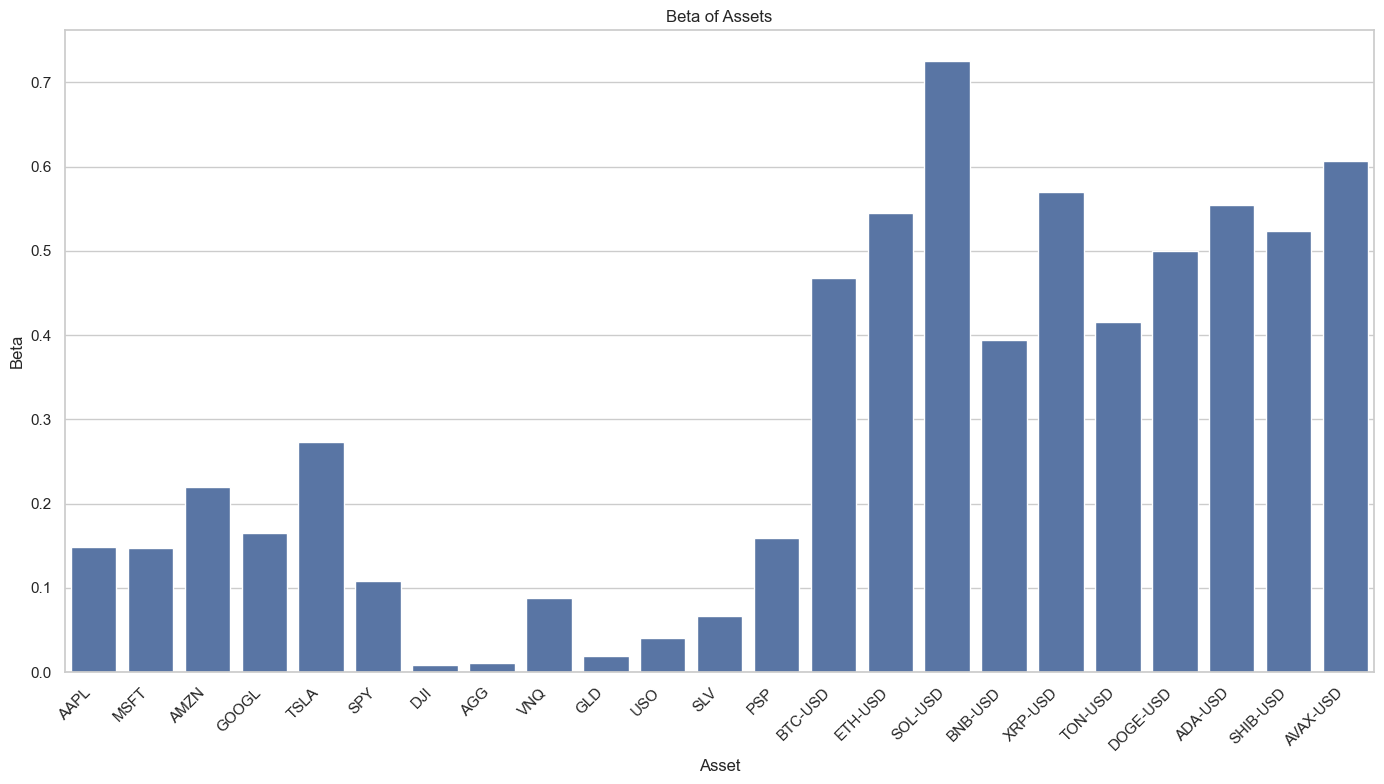
\includegraphics[width=\textwidth]{./code/risk-and-return-analysis/capm/beta_assets.png}
    \caption{Beta of Assets Relative to BITW}
    \label{fig:beta}
\end{figure}

\begin{figure}
    \centering
    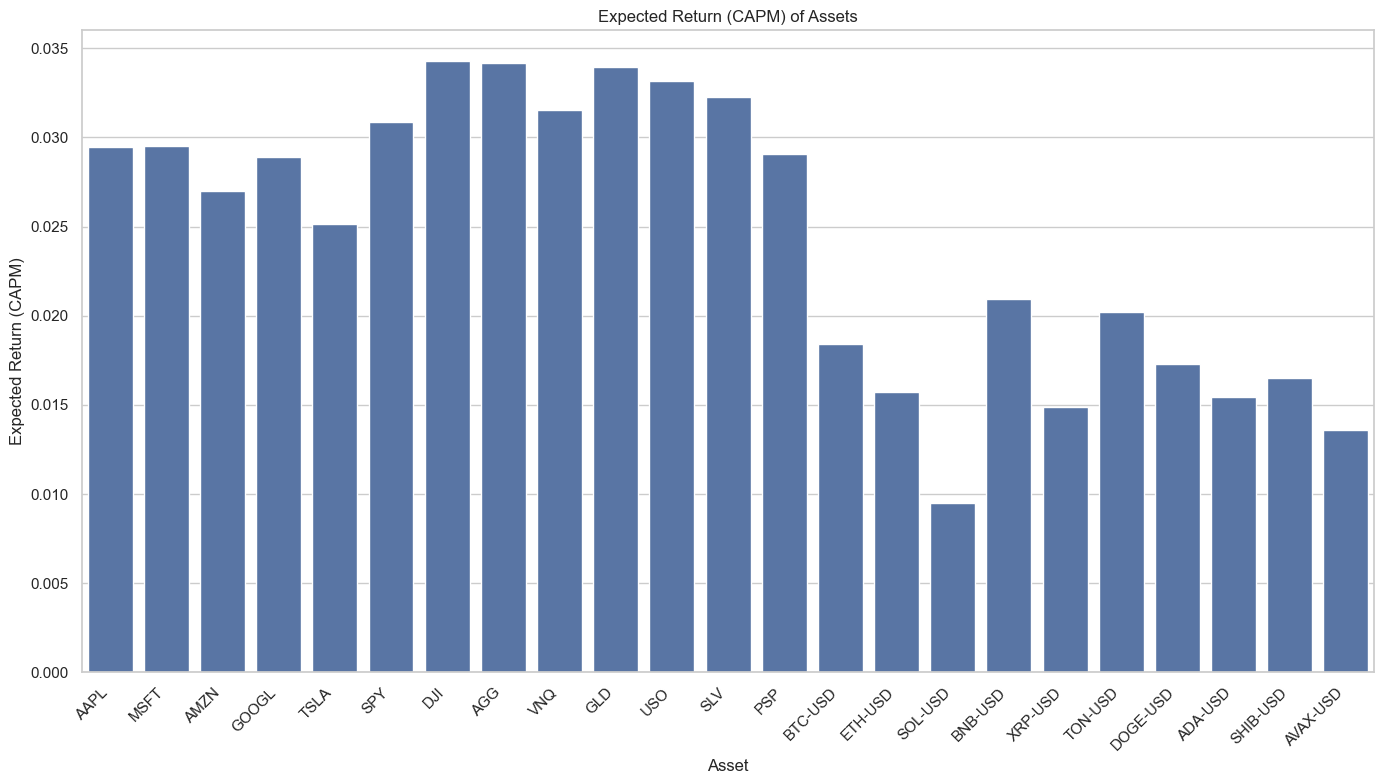
\includegraphics[width=\textwidth]{./code/risk-and-return-analysis/capm/exp_return_assets.png}
    \caption{Expected Return of Assets Relative to BITW}
    \label{fig:exp_return}
\end{figure}


\subsection{GARCH Model}

To investigate the time-varying volatility of different financial assets via the GAR Model, we first calculated the daily returns of each asset. Next, we specified and fitted a GARCH(1,1) model to the return data for each asset. This model choice is common in finance for capturing volatility clustering. After fitting the models, we evaluated their performance using various criteria. This included examining summary statistics, such as the Akaike Information Criterion (AIC) and Bayesian Information Criterion (BIC), to assess model fit and complexity. Additionally, we analyzed residuals to ensure they exhibited characteristics of white noise and conducted stationarity tests to validate model assumptions. Finally, we performed out-of-sample forecasting to assess the model's predictive ability.

\begin{figure}
    \centering
    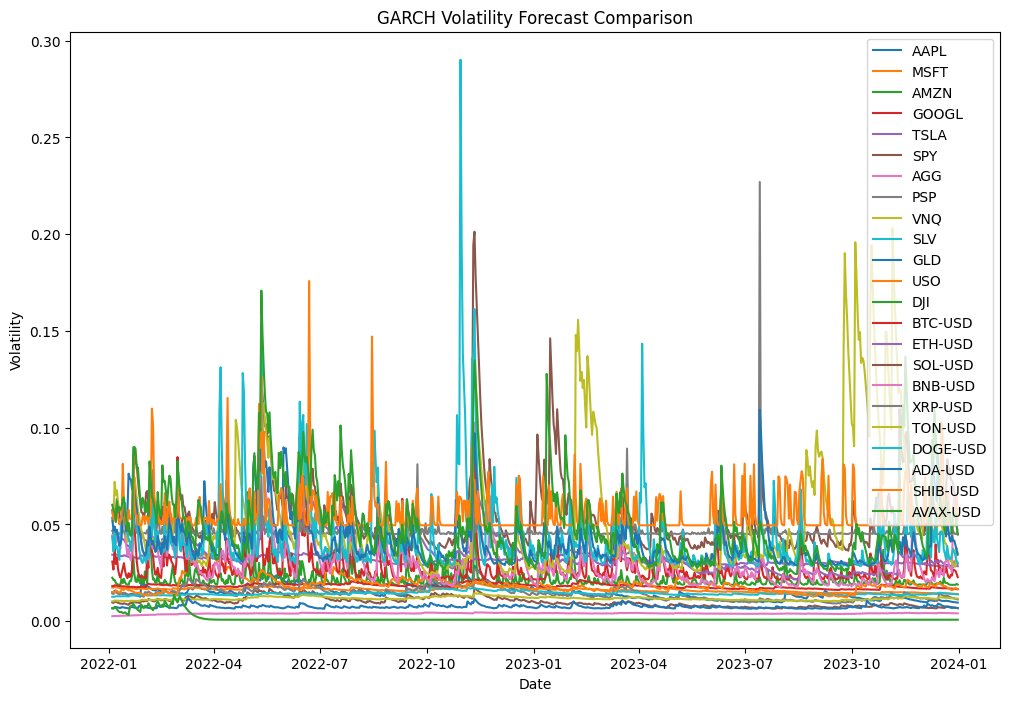
\includegraphics[width=\textwidth]{code/volatility-analysis/garch-with-mulit-assets/garch_forecast.png}
    \caption{GARCH Volatility Forecast}
    \label{fig:exp_return}
\end{figure}

\begin{figure}
    \centering
    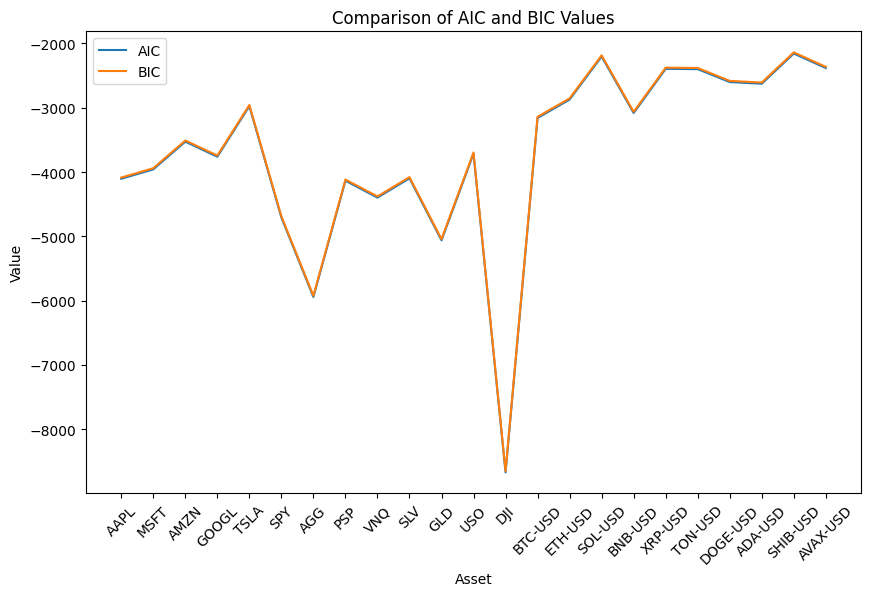
\includegraphics[width=\textwidth]{code/volatility-analysis/garch-with-mulit-assets/aic_bic.png}
    \caption{Comparison between AIC and BIC Values}
    \label{fig:exp_return}
\end{figure}

\begin{figure}
    \centering
    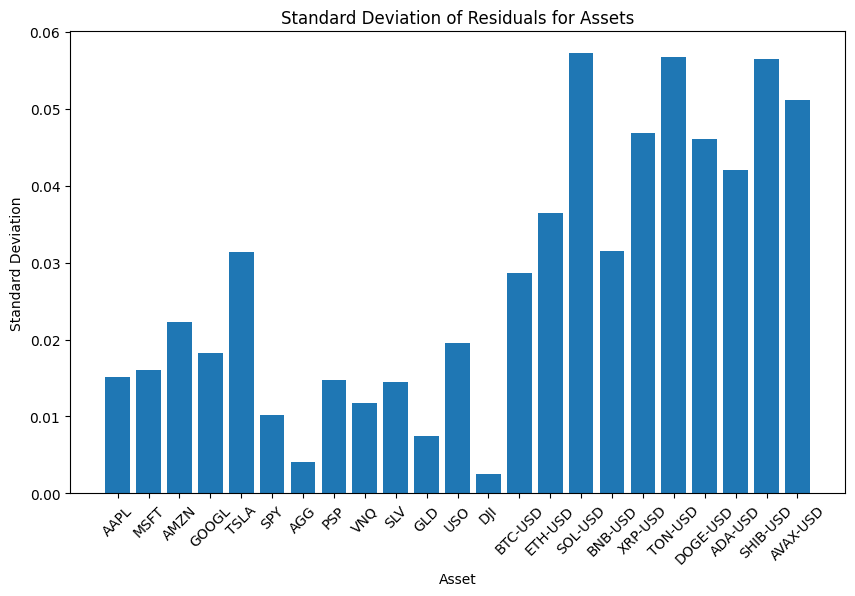
\includegraphics[width=\textwidth]{code/volatility-analysis/garch-with-mulit-assets/standard_deviation.png}
    \caption{Standard Deviation of Residuals}
    \label{fig:exp_return}
\end{figure}

\subsection{LSTM Model}

Preprocessing Steps

Historical price data for the top 10 cryptocurrencies were fetched using the yfinance library, covering the period from January 1, 2022, to January 1, 2024.

The MinMaxScaler from scikit-learn\cite{scikit-learn} was used to normalize the 'Adj Close' price data to a range between 0 and 1. This is crucial for LSTM models, which are sensitive to the scale of input data.

\subsubsection{Model Architecture and Key Values}

In our research, we developed a Bidirectional Long Short-Term Memory (LSTM) model for time series forecasting. Below is a detailed breakdown of the key values and components of our model:

\begin{itemize}
    \item {Sequence Length (SEQ\_LEN)}: 100
    \item {Dropout Rate (DROPOUT)}: 0.2
    \item {Window Size (WINDOW\_SIZE)}: \(SEQ_LEN - 1 = 99\)
    \item {Batch Size (BATCH\_SIZE)}: 64
\end{itemize}

\subsubsection{Model Layers and Structure}

\begin{enumerate}
    \item {Input Layer}:
    \begin{itemize}
        \item Shape: (WINDOW\_SIZE, Number of Features in Input)
        \item Key Value: \texttt{input\_shape = (WINDOW\_SIZE, X\_train.shape[-1])}
    \end{itemize}

    \item {First Bidirectional LSTM Layer}:
    \begin{itemize}
        \item Units: WINDOW\_SIZE = 99
        \item Return Sequences: True
        \item Key Value: \texttt{model.add(Bidirectional(LSTM(WINDOW\_SIZE, return\_sequences=True)))}
    \end{itemize}

    \item {First Dropout Layer}:
    \begin{itemize}
        \item Rate: DROPOUT = 0.2
        \item Key Value: \texttt{model.add(Dropout(rate=DROPOUT))}
    \end{itemize}

    \item {Second Bidirectional LSTM Layer}:
    \begin{itemize}
        \item Units: WINDOW\_SIZE * 2 = 198
        \item Return Sequences: True
        \item Key Value: \texttt{model.add(Bidirectional(LSTM(WINDOW\_SIZE * 2, return\_sequences=True)))}
    \end{itemize}

    \item {Second Dropout Layer}:
    \begin{itemize}
        \item Rate: DROPOUT = 0.2
        \item Key Value: \texttt{model.add(Dropout(rate=DROPOUT))}
    \end{itemize}

    \item {Third Bidirectional LSTM Layer}:
    \begin{itemize}
        \item Units: WINDOW\_SIZE = 99
        \item Return Sequences: False
        \item Key Value: \texttt{model.add(Bidirectional(LSTM(WINDOW\_SIZE, return\_sequences=False)))}
    \end{itemize}

    \item {Dense Layer}:
    \begin{itemize}
        \item Units: 1
        \item Key Value: \texttt{model.add(Dense(units=1))}
    \end{itemize}

    \item {Activation Layer}:
    \begin{itemize}
        \item Activation Function: Linear
        \item Key Value: \texttt{model.add(Activation('linear'))}
    \end{itemize}
\end{enumerate}

\section*{Model Compilation}

\begin{itemize}
    \item Loss Function: Mean Squared Error
    \item Optimizer: Adam
    \item Key Value: \texttt{model.compile(loss='mean\_squared\_error', optimizer='adam')}
\end{itemize}

\section*{Model Training Parameters}

\begin{itemize}
    \item Epochs: 50
    \item Batch Size: BATCH\_SIZE = 64
    \item Shuffle: False
    \item Validation Split: 10\%
    \item Key Value: \texttt{model.fit(X\_train, y\_train, epochs=50, batch\_size=BATCH\_SIZE, shuffle=False, validation\_split=0.1)}
\end{itemize}

\section*{Summary}

We utilized a Bidirectional LSTM model with three layers of bidirectional LSTMs, each followed by dropout layers to prevent overfitting. The final dense layer with a linear activation function is used for regression. Our model is compiled using the mean squared error loss function and the Adam optimizer, and trained over 50 epochs with a batch size of 64, using 10\% of the training data for validation.

This architecture effectively captures temporal dependencies in both directions, making it suitable for time series forecasting tasks.



\section{Volatility Analysis}

Volatility analysis plays a crucial role in understanding the behavior of financial assets, particularly in the realm of alternative investments. Volatility, often regarded as a measure of risk, encapsulates the degree of uncertainty or variability in the returns of an asset over time. In the context of alternative assets, which encompass a diverse range of investment vehicles beyond traditional stocks and bonds, volatility assumes heightened significance due to the unique characteristics and dynamics inherent in these assets.

The emergence of digital assets, such as cryptocurrencies and tokenized securities, has further underscored the importance of volatility analysis in alternative asset management. These nascent and rapidly evolving asset classes exhibit distinct patterns of price fluctuations and risk profiles, necessitating sophisticated analytical tools to model and assess their volatility dynamics accurately.

Volatility analysis serves multiple purposes in the management of alternative assets. Firstly, it provides insights into the inherent risk associated with these assets, enabling investors and portfolio managers to make informed decisions regarding asset allocation, risk mitigation strategies, and portfolio diversification. Secondly, volatility analysis facilitates the estimation of potential returns and the pricing of derivative instruments, such as options and futures, which are commonly utilized in alternative asset markets for hedging and speculation purposes.

Two prominent methodologies employed in volatility analysis are the Generalized Autoregressive Conditional Heteroskedasticity (GARCH) model and Stochastic Geometric Brownian Motion (GBM). The GARCH model, a time-series econometric framework, is widely utilized to model the volatility clustering and persistence observed in financial asset returns. By capturing the conditional heteroskedasticity of asset returns, the GARCH model enables practitioners to forecast future volatility levels accurately and assess the risk-return characteristics of alternative assets.

On the other hand, stochastic GBM, a stochastic process widely used in mathematical finance, provides a continuous-time framework for modeling the evolution of asset prices and their associated volatility. By incorporating random fluctuations and drift components into the asset price dynamics, stochastic GBM offers a versatile approach to simulating the behavior of alternative assets under various market conditions and investment scenarios.

\subsection{Stochastic Model - GBM}




\begin{table}
    \centering
    \begin{tabular}{ccc}
         \toprule
         \textbf{Asset} & \textbf{Mean} & \textbf{Standard Deviation} \\
         \midrule
         BTC-USD & 34831.378123 & 12556.081916 \\
         ETH-USD & 2186.967729 & 863.545155 \\
         SOL-USD & 55.782474 & 55.221616 \\
         BNB-USD & 323.091985 & 117.789668 \\
         XRP-USD & 0.631261 & 0.287855 \\
         TON-USD & 3.99546 & 3.533988 \\
         DOGE-USD & 0.125877 & 0.094779 \\
         ADA-USD & 0.829737 & 0.632222 \\
         SHIB-USD & 0.000013 & 0.000011 \\
         AVAX-USD & 32.960283 & 28.309159 \\
         \bottomrule
    \end{tabular}
    \caption{Summary Statistics of Selected Digital Assets}
    \label{tab:summary_stats}
\end{table}


\section{Valuation Techniques}

Valuing cryptocurrencies presents unique challenges and opportunities compared to traditional assets. The decentralized and digital nature of these assets requires innovative approaches to determine their intrinsic and market values. Below, we discuss key valuation techniques, including the collection of on-chain data and the application of relative valuation models.

\subsection{Collect On-Chain Data}

On-chain data refers to information that is recorded directly on the blockchain, the underlying technology of cryptocurrencies. This data provides valuable insights into the network's activity and health, which can be used to inform valuation models. Key metrics include transaction volume, active addresses, and the total value transacted on the network.

\subsubsection{Importance of On-Chain Data}

$ \bullet $ \textbf{Transparency}: On-chain data is publicly accessible, allowing analysts to observe real-time network activity.

$ \bullet $ \textbf{Market Sentiment}: High transaction volumes and active addresses can indicate strong market interest and adoption.

$ \bullet $ \textbf{Security and Reliability}: The decentralized nature of blockchain technology ensures that the data is tamper-proof and reliable.

\hfill \break

\subsubsection{Transaction Volume}

Transaction volume measures the total amount of cryptocurrency transferred within the network over a given period. High transaction volumes can signal increased usage and demand for the cryptocurrency, potentially leading to higher valuations.

\hfill \break

\subsection{Relative Valuation Models}

Relative valuation models compare the value of a cryptocurrency to other similar assets, providing a framework to assess whether a cryptocurrency is overvalued or undervalued relative to its peers. One of the most widely used relative valuation models in the cryptocurrency space is the Network Value to Transactions (NVT) ratio.

\hfill \break

\subsubsection{Network Value to Transactions (NVT) Ratio}

\hfill \break

The NVT ratio is akin to the price-to-earnings (P/E) ratio used in equity markets. It is calculated by dividing the market capitalization of a cryptocurrency by its daily transaction volume.

\[
\text{NVT Ratio} = \frac{\text{Market Capitalization}}{\text{Daily Transaction Volume}}
\]

$ \bullet $ \textbf{Market Capitalization}: The total value of all coins in circulation, calculated by multiplying the current price by the total supply.

$ \bullet $  \textbf{Daily Transaction Volume}: The sum of all transactions made within a 24-hour period.

\hfill \break

\subsubsection{Interpretation of the NVT Ratio}

\hfill \break

$ \bullet $  \textbf{High NVT Ratio}: Indicates that the network value (market cap) is high relative to its transaction volume. This could suggest that the cryptocurrency is overvalued or that it is being used more as a store of value rather than for transactions.

$ \bullet $  \textbf{Low NVT Ratio}: Suggests that the network is undervalued relative to its transaction volume, indicating healthy network activity and potentially higher growth prospects.

\subsection{Absolute Valuation Models}

The Equation of Exchange is given by:

\[
MV = PQ
\]

Where:

$ \bullet $  $M$ is the total money supply.

$ \bullet $  $V$ is the velocity of money.

$ \bullet $ $P$ is the price level.

$ \bullet $ $Q$ is the transaction volume (or economic output).


For cryptocurrencies:
\[
\text{Intrinsic Value} = \frac{P \times Q}{V}
\]

Results

\begin{figure}
    \centering
    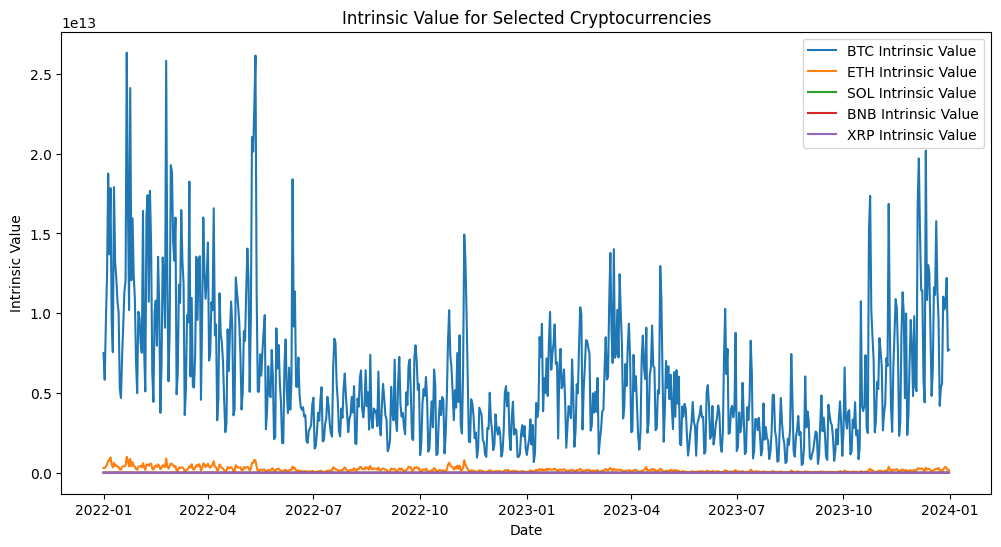
\includegraphics[width=0.8\textwidth]{./code/valuation-techniques/intrinsic_value.png}
    \caption{Intrinsic Value }
    \label{fig:beta}
\end{figure}

\begin{figure}
    \centering
    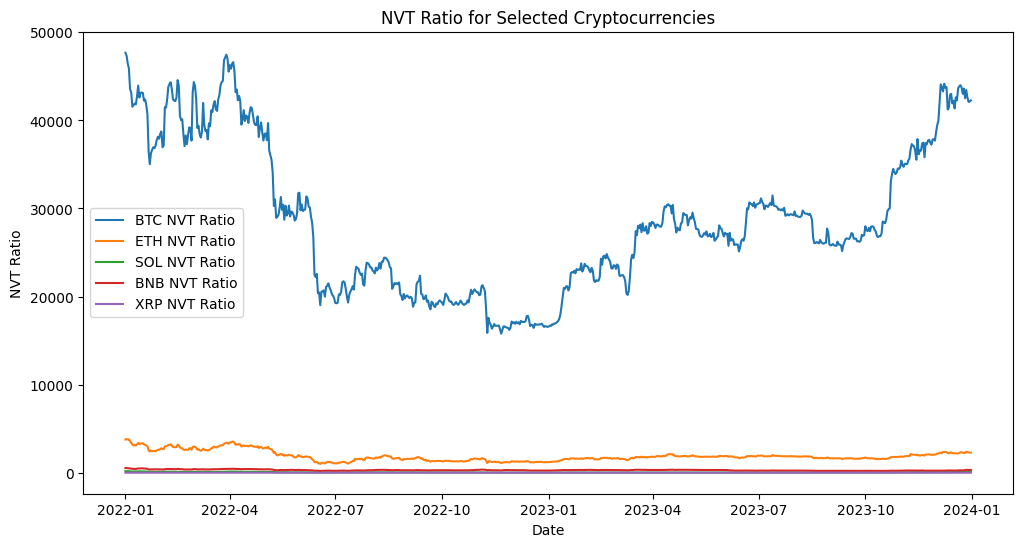
\includegraphics[width=0.8\textwidth]{./code/valuation-techniques/nvt_ratio.png}
    \caption{Network Value to Transactions Ratios}
    \label{fig:beta}
\end{figure}

We have to make some assumptions or gather data for $V$ (velocity), $P$ (price level), and $Q$ (transaction volume).

\hfill \break

\subsection{Application of Valuation Techniques to Cryptocurrencies}

By leveraging on-chain data and relative valuation models like the NVT ratio, investors and analysts can gain a deeper understanding of the intrinsic value and market dynamics of cryptocurrencies. These techniques help in identifying investment opportunities and assessing the fundamental health of different cryptocurrency networks.

In conclusion, the integration of on-chain data and innovative valuation models provides a robust framework for analyzing and valuing cryptocurrencies. As the market for digital assets continues to evolve, these techniques will play a crucial role in guiding investment decisions and fostering a deeper understanding of the complex dynamics at play.



\section{Price Prediction}

Need more info.

\section{Portfolio Management Strategies}

Need more info.

\section{Analysis}
\subsection{CAPM Analysis}

From the period measured of Jan 01, 2022 to Jan 01, 2024, we see that all assets are less than 1 to the BITW market index, meaning that they are less volatile compared to the assets in the BITW. We expect and see that the cryptocurrencies coin have betas higher than the other asset class measure. The beta is then followed by FAANG stocks like Apple, Amazon, Google. We do see PSP and VNQ within the same beta range of 0.1 - 0.2. 

More over, if we further observe, we see the expected return of all assets not-including cryptocurrencies have a high expected return between 2.5\% - 3.5\%. Cryptocurrencies fall in the range between 0.9\% and 0.22\%, incremental gains compared to the rest of the market.

Overall, we can observe that there is a significant difference in risk and return between regular assets classes like stocks, gold, real estate to cryptocurrencies. More analysis needs to be made to draw further conclusions and longer time horizons need to be observed, but the returns gained from cryptocurrencies stems differently from the returns of other assets, possibly via the different risk exposure in the market.

\subsection{GARCH Model}

- cryptocurrency are more volatile than traditional assets (standard deviation)
- AIC and BIC values are negative, with DJI being the most negative

\subsection{Relative and Absolute Valuation Techniques}

By leveraging on-chain data and relative valuation models like the NVT ratio, investors and analysts can gain a deeper understanding of the intrinsic value and market dynamics of cryptocurrencies. These techniques help in identifying investment opportunities and assessing the fundamental health of different cryptocurrency networks.

In conclusion, the integration of on-chain data and innovative valuation models provides a robust framework for analyzing and valuing cryptocurrencies. As the market for digital assets continues to evolve, these techniques will play a crucial role in guiding investment decisions and fostering a deeper understanding of the complex dynamics at play.


\subsection{NVT Model}

\subsection{Intrinsic Value Model}
-110 and 120
\subsection{LSTM Model}

%define the following sections to hide their Section Number (Notes Style)
\ledgernotes

\section*{Acknowledgements} 

We would like to express our sincere gratitude to Dr. Simon Mak for his invaluable guidance and support in both the SMU Blockchain Club and this research paper. We also wish to acknowledge the SMU Blockchain Club community for their support and collaboration, which were instrumental to this work. Special thanks go to the Engaged Learning Fellowship Program, particularly Jennifer Ebinger, Senior Director, and Adam Neal, Program Manager, for their encouragement and assistance. Lastly, we extend our heartfelt thanks to Southern Methodist University for their generous financial support.

\section*{Author Contributions}

State the contribution made by each author.  Refer to authors using their initials, for example, ``FAL developed the code to perform the simulation (65\%) and FQL analyzed the results (35\%).  They both contributed equally to manuscript preparation.''

\section*{Conflict of Interest}

Authors should state any conflict of interest as defined by Ledger's Conflict of Interest Policy, available on the Ledger website. If the author believes there are no conflicts of interest, they should include the following: ``The author declares that they have no known conflicts of interest as per the journal’s Conflict of Interest Policy.''

%AUTHOR: comment out if using thebibliography
%\theendnotes

%AUTHOR: please read ledgerbib.bst usage notes by opening it in a text editor. We have modified it to include the use of the @misc item type for the proper formatting of online sources.

\bibliographystyle{ledgerbib}
\bibliography{tempbib}

%AUTHOR: comment out, this is used to make sure the Creative Commons License
%image fits on page

\newpage 	
%define the following sections to have the Appendix Style

\appendix
\setcounter{section}{0}
\section{Capital Asset Pricing Model (CAPM) Details}\label{appendix:capm_details}

\vspace{12pt}

\begin{longtable}{|l|l|c|c|c|c|}
\hline
\textbf{Asset} & \textbf{Asset Class} & \textbf{Beta} & \textbf{Expected Return (CAPM)} & \textbf{R-squared} & \textbf{p-value} \\
\hline
AAPL & Equities & 0.1489 & 0.0294 & 0.1295 & $1.22 \times 10^{-23}$ \\
MSFT & Equities & 0.1469 & 0.0295 & 0.1127 & $1.30 \times 10^{-20}$ \\
AMZN & Equities & 0.2194 & 0.0270 & 0.1310 & $6.41 \times 10^{-24}$ \\
GOOGL & Equities & 0.1653 & 0.0289 & 0.1108 & $2.83 \times 10^{-20}$ \\
TSLA & Equities & 0.2734 & 0.0251 & 0.1018 & $1.13 \times 10^{-18}$ \\
SPY & Equities & 0.1084 & 0.0308 & 0.1519 & $8.59 \times 10^{-28}$ \\
DJI & Equities & 0.0089 & 0.0343 & 0.0176 & $3.32 \times 10^{-4}$ \\
AGG & Bonds & 0.0115 & 0.0342 & 0.0108 & 0.5081 \\
VNQ & Real Estate & 0.0884 & 0.0315 & 0.0754 & $4.80 \times 10^{-14}$ \\
GLD & Commodities & 0.0195 & 0.0339 & 0.0091 & 0.1010 \\
USO & Commodities & 0.0408 & 0.0332 & 0.0059 & 0.0387 \\
SLV & Commodities & 0.0671 & 0.0323 & 0.0291 & $3.73 \times 10^{-6}$ \\
PSP & Private Equity & 0.1596 & 0.0291 & 0.1584 & $5.26 \times 10^{-29}$ \\
BTC-USD & Cryptos & 0.4680 & 0.0184 & 0.3584 & $6.78 \times 10^{-72}$ \\
ETH-USD & Cryptos & 0.5448 & 0.0157 & 0.3008 & $2.47 \times 10^{-58}$ \\
SOL-USD & Cryptos & 0.7253 & 0.0095 & 0.2163 & $2.76 \times 10^{-40}$ \\
BNB-USD & Cryptos & 0.3944 & 0.0209 & 0.2106 & $3.79 \times 10^{-39}$ \\
XRP-USD & Cryptos & 0.5699 & 0.0149 & 0.1991 & $7.28 \times 10^{-37}$ \\
TON-USD & Cryptos & 0.4154 & 0.0202 & 0.0721 & $1.78 \times 10^{-13}$ \\
DOGE-USD & Cryptos & 0.4995 & 0.0173 & 0.1583 & $5.43 \times 10^{-29}$ \\
ADA-USD & Cryptos & 0.5541 & 0.0154 & 0.2331 & $9.96 \times 10^{-44}$ \\
SHIB-USD & Cryptos & 0.5231 & 0.0165 & 0.1156 & $3.89 \times 10^{-21}$ \\
AVAX-USD & Cryptos & 0.6062 & 0.0136 & 0.1888 & $7.68 \times 10^{-35}$ \\
\hline
\end{longtable}




\thispagestyle{pagelast}





%\theendnotes

\end{document}
